% Webservices
\chapter{Web Services}
\label{sec:webservices}

Web Services ermöglichen es, verschiedene Programme miteinander in einem Netzwerk zu verbinden. Hierfür stellen sie eine einheitliche Schnittstelle für die Kommunikation untereinander zur Verfügung. Dabei spielt die Wahl der Plattform - ob Windows, Linux oder \ac{iOS} - als auch die Wahl der Programmiersprachen wie Java, \ac{PHP} oder Python keine Rolle. Somit können einzelne Programme, Module oder Komponenten in unterschiedlichen Sprachen von unterschiedlichen Teams entworfen werden, so wie auf beliebigen Systemen installiert werden. 
\\
\linebreak
Eine der zentralen Funktionen eines Webservices ist die Synchronisation von Client und Server. Ein Webservice stellt dem Client Informationen, zum Beispiel über Datentypen, möglichen Operationen sowie die Parameter und Rückgabewerte und Hinweise darüber, wie diese Aufgerufen werden können, zur Verfügung. Für die Kommunikation ist es wichtig ein Transportprotokoll und das Format für die übertragenen Daten festzulegen. Als Transportprotokolle können beispielsweise \ac{SMTP}, \ac{TCP}, \ac{JMS}, \ac{HTTP} oder \ac{HTTPS} genutzt werden. Übliche Datenformate sind dabei \ac{XML} oder \ac{JSON}. 
\\
\linebreak
Allein mit dem Konzept der Webservices ist die Implementierung einer verteilten Anwendung jedoch nicht möglich. Denn Webservices stellen hauptsächlich Dienste und Funktionen über definierte Schnittstellen und Standards über das Netzwerk zur Verfügung, sie dienen also eher zur Kommunikation der Systeme untereinander und weniger zur Abarbeitung logischer Konzepte. Zudem bieten Webservices kein ausreichendes Maß an loser Kopplung. Wie bereits in Kapitel \ref{sec:archfazit} erwähnt wurde, werden Webservices oft im Zusammenhang mit \ac{SOA} gebracht. Dies liegt daran, dass die grundlegenden Konzepte von \ac{SOA} durch Webservices umgesetzt werden können\autocites[Vgl.][23\psqq]{jws}[Vgl.][8\psqq]{soamws}.

\section{Serviceorientierte Architektur}
\label{sec:ws_soa}

Um zu verstehen, was \ac{SOA} ausmacht und wie es verstanden werden muss empfiehlt es sich folgende Aussage zu lesen:

\begin{quote}
\glqq{}Service Oriented Architecture (SOA) is an architectural paradigm that has gained significant attention within the information technology (IT) and business communities.\grqq{} \autocite[][]{oasisspec}
\end{quote}

Eine konkrete oder einheitliche Definition für \ac{SOA} existiert derzeit nicht, deswegen wird \ac{SOA} als ein Paradigma der Architektur bezeichnet. Außerdem ist \ac{SOA} eben deswegen nicht wirklich eine Architektur, sondern eher ein Design/Konzept für verteilte Systeme. Da viele unter \ac{SOA} etwas unterschiedliches verstehen und das Paradigma meistens verschieden implementiert wird, hat die \ac{OASIS} ein \ac{SOA}-Referenzmodell definiert um es zu vereinheitlichen\autocites[Vgl.][11]{soamws}[Vgl.][2\psq]{soaidp}[Vgl.][]{oasis}.

\begin{figure}[H]
\centering
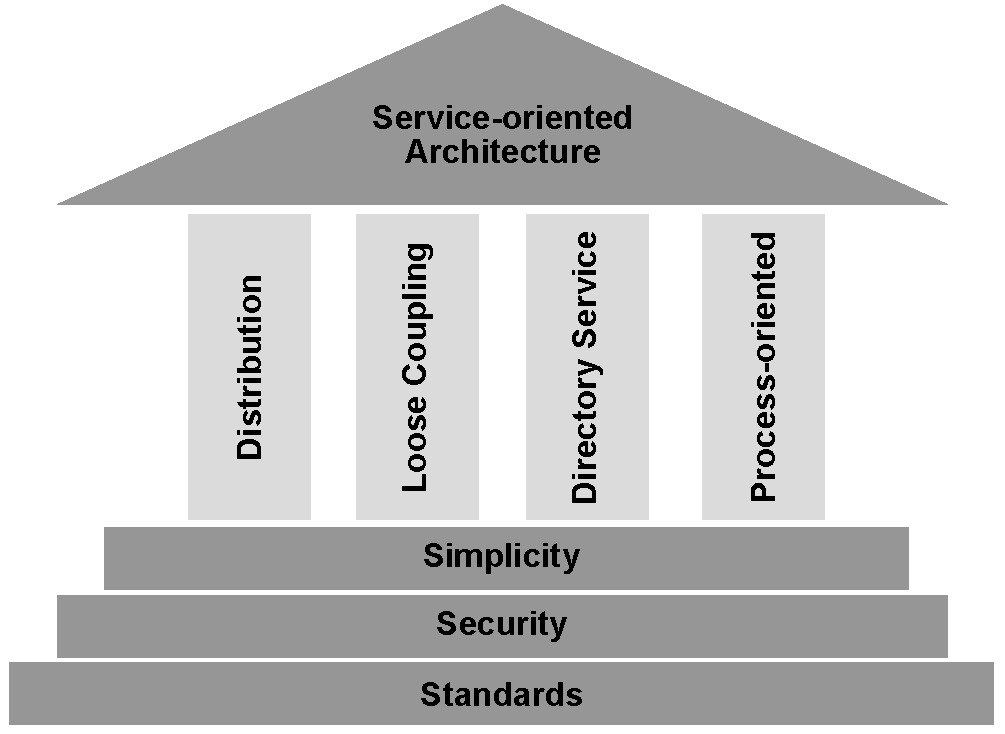
\includegraphics[width=\pictureWidth cm]{Bilder/Sonstiges/SOA_Tempel_Melzer.pdf}
\caption{SOA Tempel\label{fig:soatempel}\protect\footnotemark}%autocite[][11\psq]{soamws}}
\end{figure}
\begin{quote}
\footnotetext{Melzer (2007)}

Autor Ingo Melzer beschreibt das Grundkonzept von \ac{SOA} passend als einen Tempel, wie er in Abbildung \ref{fig:soatempel} zusehen ist, über den er folgendes sagt:

 \glqq{}Das Fundament wird von offenen Standards, Sicherheit und Zuverlässigkeit gebildet. Die verteilten Dienste, die lose Kopplung, die Plattformunabhängigkeit und die prozessorientierte Struktur sind die tragenden Säulen.\grqq{} \footnote{a.a.O., S. 11 f.}
\end{quote}

Aus diesen grundlegenden Aussagen über \ac{SOA} können einige Schlussfolgerungen abgeleitet werden. Durch das Paradigma \ac{SOA} wird die funktionale Zerlegung eines Gesamtsystems in einzelne Komponenten, genannt Services, und die Verteilung dieser auf ein Netzwerk ermöglicht. Wobei hierfür die einzelnen Services Plattform-, sprachen- und Frameworkunabhängig von einander entwickelt und wiederverwendet werden können\autocite[Vgl.][121\psq]{gmodse}.

\subsection{Technische Konzepte}
Um das Potential von \ac{SOA} nutzen zu können, werden verschiedene technische Konzepte verwendet. Die wichtigsten technischen Konzepte von \ac{SOA} sind folgende\autocite[Vgl.][11]{soaidp}:

\begin{itemize}
\item \subsubsection*{Interoperabilität} Unter Interoperabilität ist die Sicherstellung der Kommunikation unterschiedlichen Systemen ohne großen Aufwand miteinander gemeint - mit den Fokus auf den Datenfluss.
\item \subsubsection*{Services} Services dürfen nicht mit Webservices verwechselt werden. Webservices sind ein technisches Konzept zur Umsetzung der Kommunikation in \ac{SOA}, wobei Services in \ac{SOA} funktionale Komponenten sind\autocite[Vgl.][123\psq]{gmodse}.
\item \subsubsection*{Lose Kopplung} Wurde bereits in Unterkapitel \ref{sec:prinzipien} ausführlich behandelt.
\end{itemize}

\subsection{Zusammenfassung}
\label{ws:zf}
Die Service orientierte Architektur mit Unterstützung von Web Services bietet eine gute Voraussetzung für die Abdeckung der nicht-funktionalen Anforderungen sowie der Prinzipien für eine Softwarearchitektur aus Kapitel \ref{sec:architektur}. An folgender Stelle wird genauer erläutert, welche nicht-funktionalen Anforderungen vorhanden sind und warum diese von \ac{SOA} in Kombination mit Webservice-Ansätzen erfüllt werden:

\begin{itemize}
\item \subsubsection*{Skalierbarkeit} 
Durch die Implementierung der Anwendung als verteiltes System kann diese auf einen beliebigen Server mit den benötigten Ressourcen ausgelagert werden. Sollten die Ressourcen irgendwann unvorhergesehen nicht mehr ausreichen, kann die Anwendung auf einen anderen Server ausgelagert werden, ohne eine Beeinflussung der Funktionalitäten der Anwendung zu erzwingen. Eine weitere Möglichkeit hierfür ist die Auslagerung der Anwendung in eine Cloud, diese Vorgehensweise ist auch als \ac{IaaS} bekannt. Unter \acp{IaaS} sind Cloud-Computing-Plattformen gemeint, die Speicher und Rechenleistung auf den Servern für die Benutzer zur Verfügung stellen. Einer der bekanntesten \acp{IaaS} ist der \ac{AWS}. Durch die Auslagerung der Anwendung auf die \ac{AWS}-Cloud wird das Management Werkzeug \textit{Elastic Beanstalk} für den Benutzer zur Verfügung gestellt. Das Elastic Beanstalk übernimmt automatisch das Management über die Bereitstellung zusätzlicher Kapazitäten, Lastenverteilung sowie die Skalierung\autocite[Vgl.][]{aws}.
\\
\linebreak
%AWS https://docs.aws.amazon.com/de_de/elasticbeanstalk/latest/dg/Welcome.html
Eine weitere Möglichkeit dafür, die Skalierbarkeit zu erhöhen, bieten Docker Container. Die Anwendung kann ebenso wie auf mehrere Server auch in einen Docker Container verschoben werden. Die Container lassen sich leicht von einem System auf ein anderes übertragen, benötigen weniger Ressourcen als virtuelle Maschinen und sollten zusätzliche Instanzen der Anwendung benötigt werden, dann können einfach neue Container gestartet werden. Sobald diese nicht mehr benötigt werden, können diese ebenso wieder gestoppt werden\autocite[Vgl.][]{docker}. Somit steht der Skalierbarkeit der Anwendung nichts im Wege.

\item \subsubsection*{Performance} 
Generell gilt, dass die Ladezeiten einer Anwendung in der Regel nicht länger als Drei Sekunden dauern dürfen. Die Performance von \ac{SOA} hängt zunächst von unterschiedlichen Faktoren ab. Manche können eher gut beeinflusst und optimiert werden, andere eher weniger. Die heutige Technologie ist ausreichend ausgereift für die Implementierung schneller und effizienter verteilter Anwendungen. Ein Beispiel dafür ist der weltbekannte Streaming-Anbieter Netflix, der bereits die erwähnten \acp{IaaS} von \ac{AWS} verwendet. Die Filme oder Serien lassen sich in Echtzeit in beliebiger Auflösung streamen\autocite[Vgl.][]{netflix}.
%https://aws.amazon.com/de/solutions/case-studies/netflix/
Außerdem ermöglicht \ac{SOA} bei einem unerwartet hohen Zugriff immer noch das Management der Lastenverteilung der einzelnen Komponenten. Somit wird die Performance durch höhere Auslastungen der Anwendung nicht beeinflusst.

\item \subsubsection*{Verfügbarkeit} 
Eine Anwendung soll im Idealfall permanent erreichbar sein. Ein hohes Maß an Verfügbarkeit kann durch \ac{SOA} erbracht werden. Durch die Replikation der Anwendung auf mehreren Servern, als \ac{IaaS} oder durch Auslagerung in den Docker-Container, kann bei einem Ausfall einer Instanz eine andere Instanz verwendet werden.

\item \subsubsection*{Sicherheit} 
Sicherheit ist einer der Wichtigsten Aspekten in einer Software, denn auch für die Anwendungen, die keine vertraulichen Informationen beinhalten, sollte immer einer Sicherheitskonzept entworfen werden. Bei einer Absicherung eines Webservices spielen folgende Aspekte eine wichtige Rolle:
\begin{itemize}
\item Authentifizierung
\item Autorisierung
\item Integrität
\end{itemize}
Es ist nicht unmöglich eine sichere Service-orientierte Architektur zu konzipieren, dennoch muss dafür frühzeitig auf die Sicherheitsaspekte eingegangen werden. Zu diesen Themen existieren bereits eine Reihe bewährter Technologien, Techniken und Standards um Webservices sicherer zu gestalten\autocite[Vgl.][188\psq]{soamws}.
\\
\linebreak
Um die Vertraulichkeit im Nachrichtenaustausch aufbauen zu können, können verschiedene Methoden des symmetrischen oder asymmetrischen Verschlüsselungsverfahren verwendet werden. Außerdem sind folgende Standards in Webservices bereits etabliert und erleichtern die Implementierung der Sicherheitsaspekte enorm:\footnote{Vgl. a.a.O., S. 190 f.; Vgl. a.a.O., S. 208 ff.}
\begin{itemize}
\item WS-Security
\item WS-Policy
\item WS-Trust
\item WS-SecureConversation
\item WS-Privacy
\item WS-Federation
\item WS-Authorization
\end{itemize}
Wie die Authentifizierung, Autorisierung und Vertraulichkeit in einem Web\-service gewährleistet werden kann, wird ausführlicher in der Bachelorarbeit zur Planung der Nutzerverwaltung und des Frontends der Stundenplan-\ac{App} der Hochschule Hof behandelt\autocite[Vgl.][]{andreasba}. 

\item \subsubsection*{Wartbarkeit} 
Die Wartbarkeit ist einer der Wichtigsten nicht-funktionalen Anforderungen, denn in der Praxis ist es oft der Fall, dass die Anforderungen an die Anwendungen sich mit der Zeit ändern oder neue Funktionalitäten hinzu kommen. Außerdem werden des öfteren erst nach einiger Zeit Fehler in der Anwendungen erkannt, die während der Entwicklung verborgen geblieben sind. Durch die modulare und flexible Gestaltung der Services in einer \ac{SOA} sind diese leicht Austausch- oder Änderbar.
\end{itemize}

Im weiteren Verlauf wird nun erläutert, welche Prinzipien der Softwarearchitektur durch \ac{SOA} in Verbindung mit Webservice-Ansätzen bereits von Beginn an gegeben sind.

\begin{itemize}
\item \subsubsection*{Kapselung} 
Services stellen eine definierte Schnittstelle für den Zugriff bereit, jedoch sind die genauen Details der Implementierung für den Benutzer unsichtbar\autocite[Vgl.][13]{soamws}.
\item \subsubsection*{Lose Kopplung} 
Die Services können auf verschiedenen Systemen in verschiedenen Programmiersprachen realisiert werden, dadurch wird die Kopplung zwischen den Hardware- und Softwareebenen verringert.
\item \subsubsection*{Modularisierung} 
Durch die Trennung der logischen Funktionalitäten in einzelne Komponenten und der Verteilung dieser auf verschiedene Services werden die Abhängigkeiten der Komponenten reduziert. Außerdem entsteht eine fachliche Trennung der Funktionalitäten. 
\item \subsubsection*{Layering} Die Umsetzung von Service-orientierten Architekturen kann in mehreren \\Schichten realisiert werden, die bereits in Abbildung \ref{fig:schichten} zu sehen waren und im Kapitel \ref{sec:schichtenarchitektur} detaillierter beschrieben werden.
\end{itemize}

Somit bietet die Service-orientierte Architektur mit Webservices einen idealen Ansatz für die Umsetzung einer sicheren und zukunftsfähigen Hochschul-\ac{App}. Jedoch kann die Realisierung von Webservices nochmals durch zwei Arten unterschieden werden, \ac{SOAP} und \ac{REST}.


\section{Webservice Arten}
In den weiteren Unterkapiteln werden die beiden Webservice Arten kurz erklärt und anhand einer Entscheidungsmatrix gegenübergestellt und bewertet. Zu unterscheiden ist, dass \ac{SOAP} ein definiertes Netzwerkprotokoll ist, das auf \ac{XML} basiert. \ac{REST} ist hingegen ein \textit{Webservice-Light-Technologie} Architekturstil, der sich nur auf das Kommunikationsprotokoll \ac{HTTP}, respektive \ac{HTTPS}, beschränkt und meisten mit dem \ac{JSON}-Datenformat in Verbindung gebracht wird\autocite[Vgl.][23\psqq]{jws}.

\subsection{Simple Object Access Protocol (SOAP)}

\begin{quote}
\glqq{}[Simple Object Access Protocol] provides a simple and lightweight mechanism for exchanging structured and typed information between peers in a decentralized, distributed environment using XML.\grqq{} \autocite[][]{w3soa}
%https://www.w3.org/TR/2000/NOTE-SOAP-20000508/
\end{quote}
\ac{SOAP} wurde durch das \ac{W3C} als industrieller Standard definiert, in dem es in drei wesentlichen Teile aufgeteilt ist:
\begin{itemize}
\item \subsubsection*{SOAP Envelope} 
Der \ac{SOAP}-Envelope definiert ein Framework, das beschreibt, was in einer Nachricht enthalten ist, wer damit umgehen sollte, und ob gewisse Parameter optional oder obligatorisch sind. Die \ac{SOAP} Nachricht besteht aus einem Envelope, einem Header und einem Body und ist als \ac{XML}-Dokument realisiert. Es wird dadurch versucht für alle Systeme den gleichen Sprachsatz zu definieren - für Anfragen und Antworten. Somit können Nachrichten mit beliebigem \ac{XML}-Inhalt ausgetauscht werden\autocite[Vgl.][]{w3soa}.
%übersetzt aus https://www.w3.org/TR/2000/NOTE-SOAP-20000508/
Durch die Trennung des Bodies vom Header entsteht eine saubere Trennung zwischen den Anwendungsdaten und Webservice spezifischen Daten\autocite[Vgl.][63\psq]{jws}

\item \subsubsection*{SOAP Encoding Regeln} 
Diese Regeln definieren einen Serialisierungsmechanismus, mit dem anwendungsdefinierte Datentypen zwischen den Services ausgetauscht werden können. Wobei hier anzumerken ist, dass \ac{XML} eine sehr flexible Codierung von Daten ermöglicht. Die unter dem \ac{W3C} beschriebenen Kodierungsregeln können in Verbindung mit der \ac{RPC}-Darstellung verwendet werden\autocite[Vgl.][]{w3soa}.
%übersetzt aus https://www.w3.org/TR/2000/NOTE-SOAP-20000508/

\item \subsubsection*{SOAP RPC-Darstellung} 
Eines der Entwurfsziele von \ac{SOAP} besteht darin, \ac{RPC}-Aufrufe unter Verwendungen der Erweiterbarkeit und Flexibilität von \ac{XML} zu kapseln und auszutauschen\footnote{ebd.}.
%übersetzt aus https://www.w3.org/TR/2000/NOTE-SOAP-20000508/
Bei der Verwendung von \ac{SOAP} durch \acp{RPC} sind folgende Transportprotokollbindungen möglich\autocite[Vgl.][85\psq]{soamws}:
\begin{itemize}
\item \ac{TCP}
\item \ac{HTTPS}
\item \ac{SMTP}
\item \ac{FTP}
\item \ac{JMS}
\item \ac{RMI}
\end{itemize}

\end{itemize}

Ein weiterer industrieller Standard des \ac{W3C} ist die \ac{WSDL}. Diese stellt ein Model und ein \ac{XML}-Format zur Beschreibung der Webservices bereit. Zusammen mit \ac{SOAP} entsteht eine Grundlage für Webservice Anwendungen\footnote{Vgl. a.a.O., S. 101 f.}.
Jedoch hat die Realität gezeigt, dass \ac{SOAP} weder leicht in der Umsetzung ist, noch tatsächlichen Zugriff auf die Objekte bietet, es ist somit eher ein Kommunikationsprotokoll für Webservice Anwendungen. Durch die Bindung von unterschiedlichen Transportprotokollen, können unterschiedliche Arten von verteilten Anwendungen mit Hilfe von \ac{SOAP} entwickelt werden. Das Problem bei \ac{SOAP} besteht darin, dass eine \ac{SOAP} Nachricht mit dem \ac{XML}-Datenformat unnötig viel Overhead produziert. Für einen einfachen, beispielhaften Request an die Hochschul-\ac{App}, wie \lstinline[columns=fixed]{getAllLectures},%[ 
die keine Parameter und keinen Body enthalten, muss dennoch ein Body definiert werden. Bei einem kleinen Datendurchsatz stellt dies noch keine Probleme dar, jedoch wird es mit Steigerung der Daten problematisch, kompliziert und ineffizient\autocite[Vgl][57\psq]{jws}.
\\
\linebreak
Aus diesem Grund wurde im Jahr 2000 durch Roy Thomas Fielding ein vereinfachter Architekturstil namens \ac{REST} eingeführt, der, wie bereits am Anfang des Kapitel erwähnt wurde, auf das \ac{JSON}-Datenformat und das Kommunikationsprotokoll \ac{HTTPS} basiert\autocite[Vgl][77\psq]{jws}.

\subsection{Representational State Transfer (REST)}
\ac{REST} hat seinen Ursprung bereits vor den Webservices, denn es wurde damals versucht die jetzt unter \ac{REST} bekannten Prinzipien als Architekturleitpfad für das Internet zu verwenden. Durch Roy Thomas Fielding wurde \ac{REST} mit Webservices kombiniert und damit eine neue Revolution von der Prinzipien ausgelöst. Von nun an war \ac{REST} auch unter dem Namen RESTful Webservice oder RESTful Web-\ac{API} bekannt. Die Webseite \textit{www.programmableweb.com} bietet eines der größten Archive für Web-\acp{API} im Internet an. Im Juli 2019 hat die Webseite eine Statistik für den Wachstum des Web-\ac{API} Archivs seit 2005 veröffentlicht\autocite[][]{apiarchive}.

\begin{figure}[H]
\centering
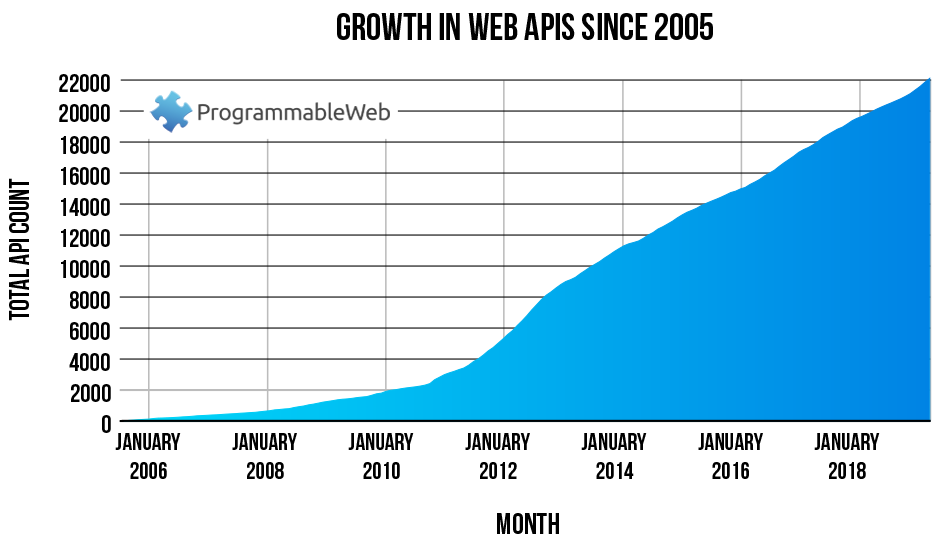
\includegraphics[width=\pictureWidth cm]{Bilder/Statistik/ProgrammableWebApis.png}
\caption{Wachstum der ProgrammableWeb API Archive von 2005\label{fig:api_statistic}\protect\footnotemark}
\end{figure}
\footnotetext{ebd.}
%https://www.programmableweb.com/news/apis-show-faster-growth-rate-2019-previous-years/research/2019/07/17

Anhand der Statistik in Abbildung \ref{fig:api_statistic} ist deutlich zu erkennen, dass die Anzahl von Web-\acp{API} seit 2006 kontinuierlich steigt. Das Potential von \ac{REST} wurde schnell erkannt, obwohl \ac{REST} immer noch - im Gegensatz zu SOAP - kein industrieller Standard, sondern eher eine Richtlinie ist, die die möglichen Nachteile von SOAP umgehen soll. Genauere Ansätze und die erwähnten Richtlinien zu \ac{REST} werden noch im Kapitel \ref{sec:ms} beschrieben.

\subsection{Bewertung}

Die folgende Entscheidungsmatrix \ref{tab:restvssoap} dient dazu, die beiden Webservice Arten gegenüberzustellen und eine Entscheidung darüber zu treffen, welche der Webservice Arten besser für die Hochschul-\ac{App} geeignet ist.

\begin{table}[H]
\begin{center}
  \begin{tabular}{| l | c | c |}
    \hline
    \rowcolor{Gray}
    \textcolor{white}{\textbf{Kriterien}} & \textcolor{white}{\textbf{REST}} & \textcolor{white}{\textbf{SOAP}} \\ \hline
    Unterstützung leichtgewichtiger Clients 		& 1 			& 0 \\
    \hline
\rowcolor{LGray}    
    Geringere Komplexität 						& 1 			& 0 \\
    \hline
    Effizienz			 						& 1 			& 0 \\
    \hline
    \rowcolor{LGray}
    Unterstützung unterschiedlichen Datenformate	& 1 			& 1 \\
    \hline
    Caching-Mechanismen	 						& 1 			& 0 \\
    \hline
    \rowcolor{LGray}
    Industrieller Standardisierung				& 0 			& 1 \\
    \hline
    Unterschiedliche Kommunikationsprotokolle		& 0 			& 1 \\
    \hline
    \rowcolor{LGray}
    Sicherheit			 						& 1 			& 1 \\
    \hline
   	\textbf{Ergebnis}							& \textbf{6}			& \textbf{4} \\
    	\hline
    	
  \end{tabular}
  \end{center}
\caption[Entscheidungsmatrix SOAP und REST]{Entscheidungsmatrix}
\label{tab:restvssoap}
\end{table}

Bedeutung der Bewertungszahlen: 
\begin{itemize}
\item \textbf{1:} trifft zu
\item \textbf{0:} trifft nicht zu
\end{itemize} 

\ac{REST} schneidet mit 2 Punkten besser als \ac{SOAP} ab. Aus diesem Grund und vor allem, da \ac{REST} für leichtgewichtige Clients wie Browser oder Smartphones entwickelt wurde und auch leichter für diese zu implementieren ist, da der ganze Overhead entfällt und es zahlreiche Caching-Mechanismen unterstützt werden, geht \ac{REST} als Sieger für die Entwicklung der Hochschul-\ac{App} hervor. Somit stellt \ac{REST} eine interessantere Grundlage für das Design der Hochschul-\ac{App} dar.
\\
\linebreak
Um die Entscheidungsmatrix und die aufgeführten Punkte, die für \ac{REST} sprechen, zu verstehen, wird im nächsten Kapitel näher  auf die beschriebenen Merkmale und Richtlinien von \ac{REST} eingegangen.